\documentclass[12pt,a4paper]{article}
\usepackage{graphicx}
\begin{document}
	\begin{titlepage}
		
		\centering
		\vspace*{\fill}
		
		\vspace*{0.5cm}
		
		\huge\bfseries
		\rule{\textwidth}{1.6pt}\\[\baselineskip]
		Thutong LMS\\ User Manual
		
		\vspace*{0.5cm}
		
		\large Edited by: \\[\baselineskip]
		
			{Fiwa Lekhulani\\Lebogang Ntatleng\\Lesego Mabe\\Tlou Lebelo}
		
		\rule{\textwidth}{1.6pt}\\[\baselineskip]
		
		
		\vspace*{\fill}
	\end{titlepage}


	\date{\textbf{\today}}
	\pagenumbering{roman}
	%\noindent\rule{\textwidth}{1pt}
	\pagebreak
	\tableofcontents
	\newpage
	\pagenumbering{arabic}


	\section{Product Overview}
		The Thutong Site Learning Center is an online system intended for high school students. It is aimed at providing students with online material to catch up on any content that they might have missed in class or did not comprehend during class. it is also aimed at providing teachers a way of uploading course content to the system for students to go through, and provide quizzes for the students to test their knowledge after the completion of a topic. 
	
	\section{System Configuration}
		The Thutong Site Learning Center system need not be installed on any any digital device, it is available online. The system can be accessed through desktop computers and mobile devices. Users will need a network connection in order to access the system. 
		
		%NOTE:please load an image here!!!
		
	\section{Installation}
		The system does not need to be installed as mentioned above, the user need only have a digital device with an internet connection and a web browser.
		
	\section{Getting Started}
		The Thutong system is aimed at improving South Africa's Science ratings, this means that it is intended to be used by every student in South Africa, thus it is free and no license is needed to use it.\\
		There are 4 types of users in the Thutong system, these are:
		\begin{itemize}
			\item Guest users
			\item Students
			\item Expert Consultants(Teachers)
			\item Administrator\\
		\end{itemize} 
		
		Some things to keep note of while using the Thutong system are:
		\begin{itemize}
			\item Administrators will be able to determine and limit certain features and functionalities that all users are exposed to throughout the system.
			\item Teachers, with the roles or "powers" assigned to them by the administrator will be able to limit the amount of content students(enrolled or not) are exposed to.
			\item The administrator will be able to customise the look and feel of the website, along with the method and style of authentication.
			\item The decision to make a course or activity available to all users is at the Administrator and/or teachers discretion. 
		\end{itemize} 
		  
		\subsection{Entry Pages}
			All users, returning or first time users are met with the welcome page depicted by Figure 1 below, when visiting the system. On this page, users are exposed to courses that are available at the moment. An option to login or register is situated at the top right corner if they wish to view content.
			
			\begin{figure}[h]
				\centering
				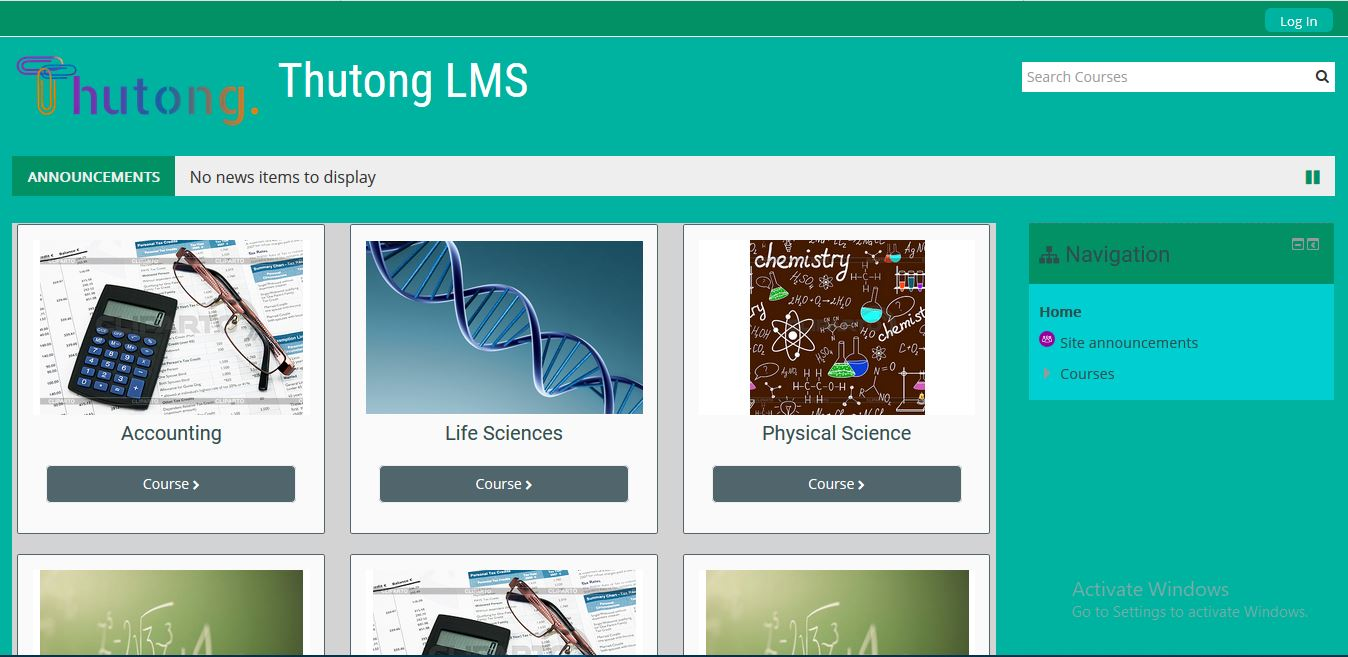
\includegraphics[width=1\textwidth]{images/welcome.JPG}
				\caption{Welcome Page}
				\label{Figure 1}
			\end{figure}
			
			\subsubsection{Login}
				Users who have already registered on the site, or alternatively were registered by the administrator can use the form on login page in Figure 2 to login as shown. On successful login they will be redirected to a different page depending on the type of user.
				
				\begin{figure}[h]
					\centering
					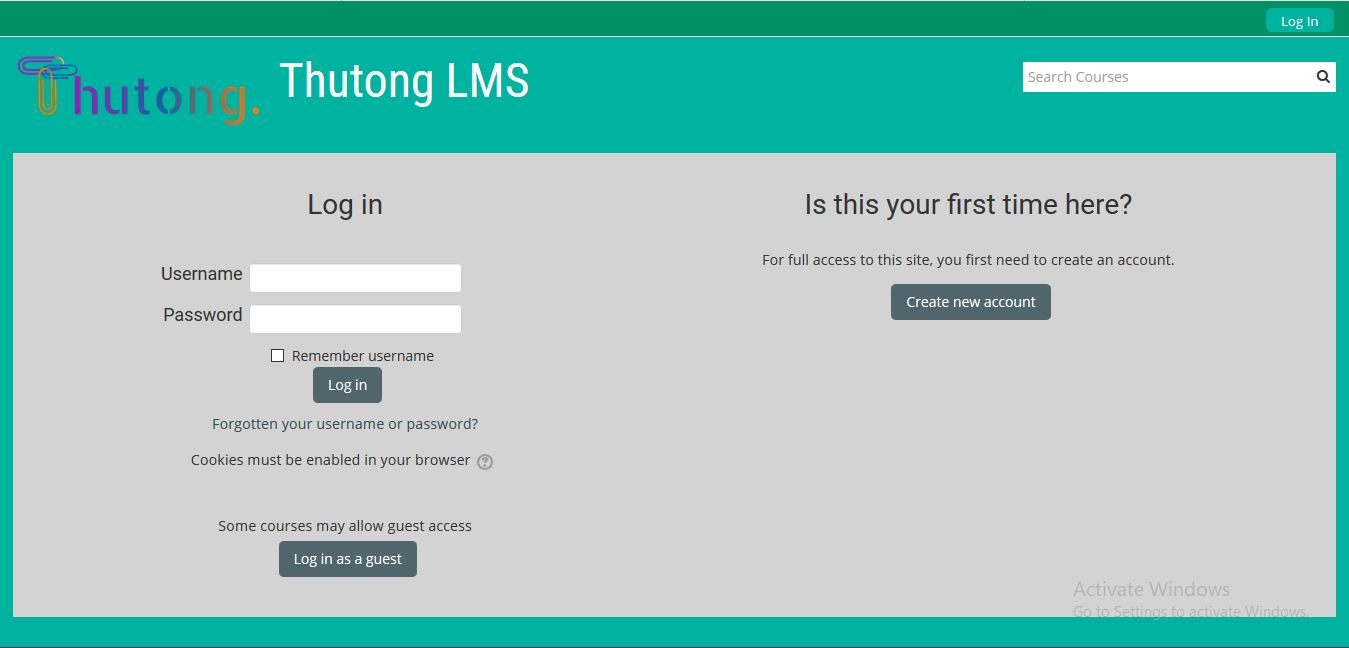
\includegraphics[width=1\textwidth]{images/login.JPG}
					\caption{Login Page}
					\label{Figure 2}
				\end{figure}
			
			\subsubsection{Registration}
				Visitors who would like to have access to courses that require authenticated users may register by clicking "Create a new account" on the login page above, where they will be taken to Figure 3 below. Here they input their credentials and upon successful registration be taken to the home page.
				
				\begin{figure}[h]
					\centering
					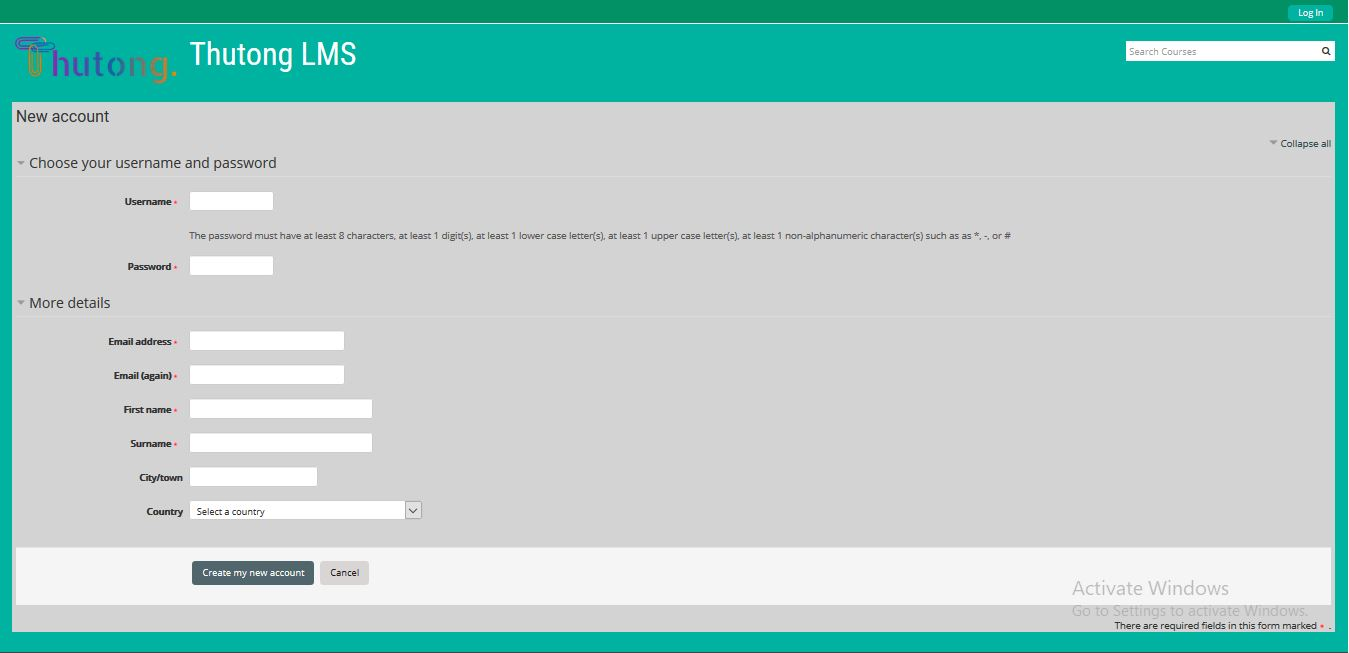
\includegraphics[width=1\textwidth]{images/registration.JPG}
					\caption{Registration Page}
					\label{Figure 3}
				\end{figure}
			
			\subsubsection{Guest Login}		
				To login as guests, visitors must click the "Login as guest" button on Figure 2 above, where they will be redirected to the default guest-login page. Here users will be able to see all courses but may only have access to courses that allow guest access, these are indicated by the circled icon on the bottom right corner of the course.
				
				\begin{figure}[h]
					\centering
					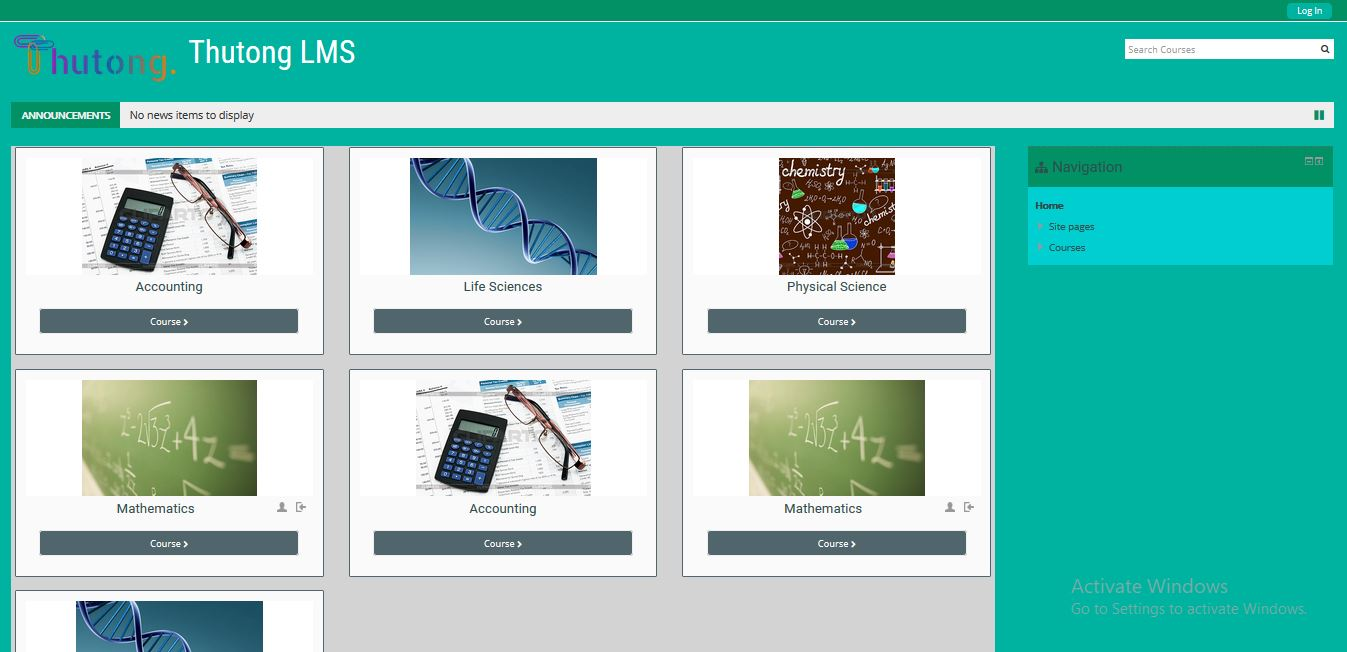
\includegraphics[width=1\textwidth]{images/guestLogin.JPG}
					\caption{Guest Login Welcome Page}
					\label{Figure 4}
				\end{figure}
			
			\subsubsection{Forgotten Passwords \& User-names}
				In the event that a user is unable to login due to a forgotten password or username, the user may click on "Forgotten your username or password?". From hereon, the user will be redirected to the page depicted by Figure 5 below.\\ \\They can then search for their accounts based on their username or email address. If either of the 2 result in a successful search, a system generated email will be sent to the email address on record where users will get a password reset link.\\
				
				\begin{figure}[!]
					\centering
					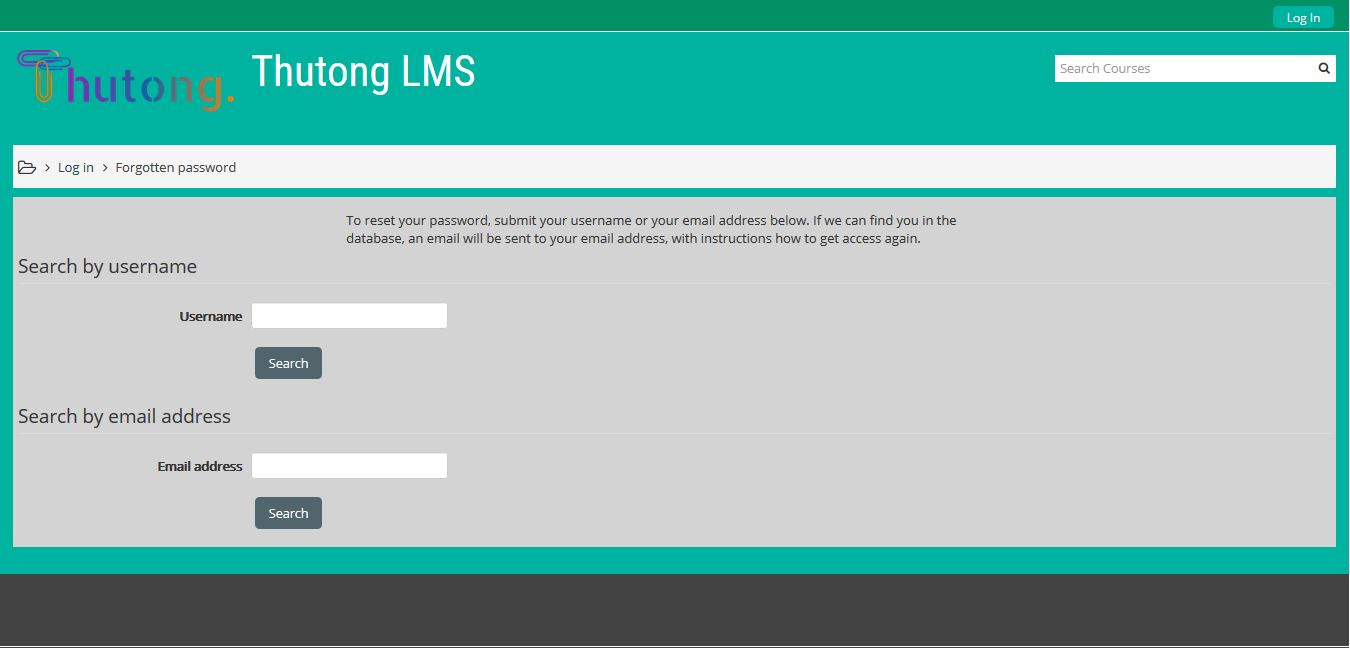
\includegraphics[width=1\textwidth]{images/forgotPassword.JPG}
					\caption{Forgotten Passwords or User-names}
					\label{Figure 5}
				\end{figure}
				 
%	\section{The Student}
%		As student, upon successful login you will be taken to the following page on Figure 6.
		
			
	\section{The Expert Consultant(Teacher)}
		The Expert consultant needs to be able to, besides logging in, add course content intended for students on the system. They should also be able to create quizzes for students and be able to remove all of the above-mentioned entities.\\Once logged in, the teacher will be taken to the following page:
		
		\begin{figure}[h]
			\centering
			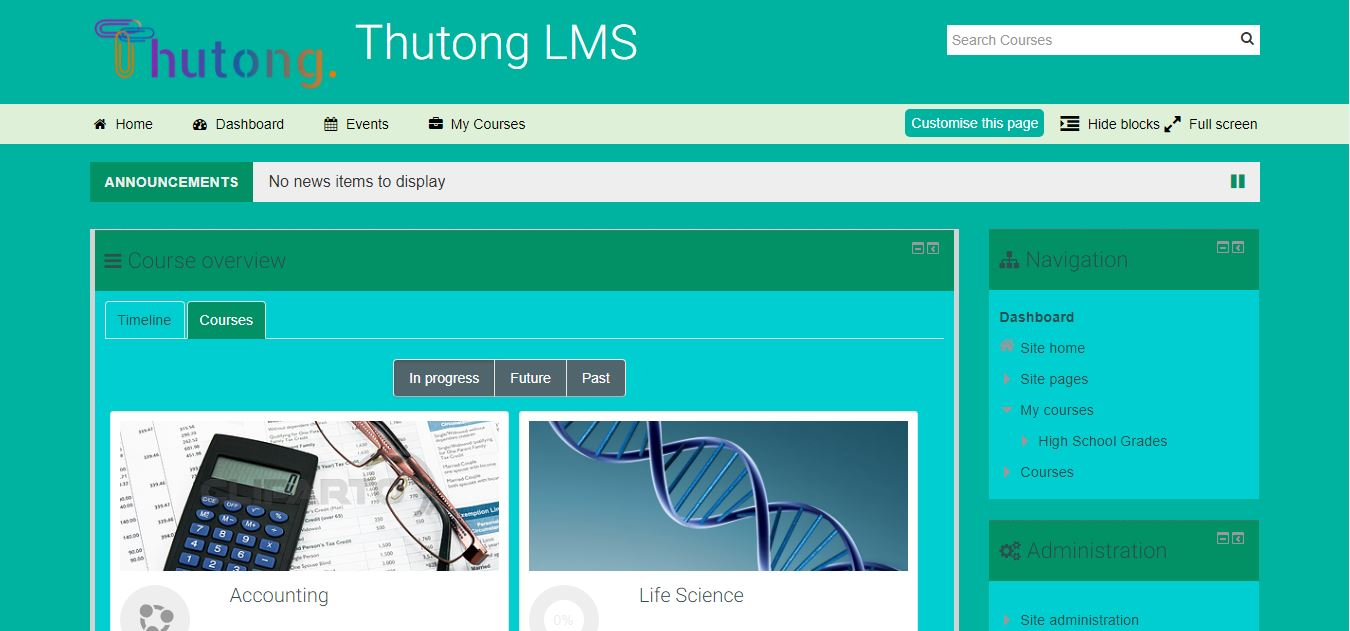
\includegraphics[width=1\textwidth]{images/teacherDash.JPG}
			\caption{Teacher Dashboard}
			\label{Figure 6}
		\end{figure}
		\subsubsection{Adding a lesson}
			In order to add a lesson, one should click "turn on editing" button to be able to edit the course. Note this is only possible if the teacher created, or was assigned previledges to manage the course. Below is the page that will load thereafter:
		 
			\begin{figure}[h]
			 	\centering
			 	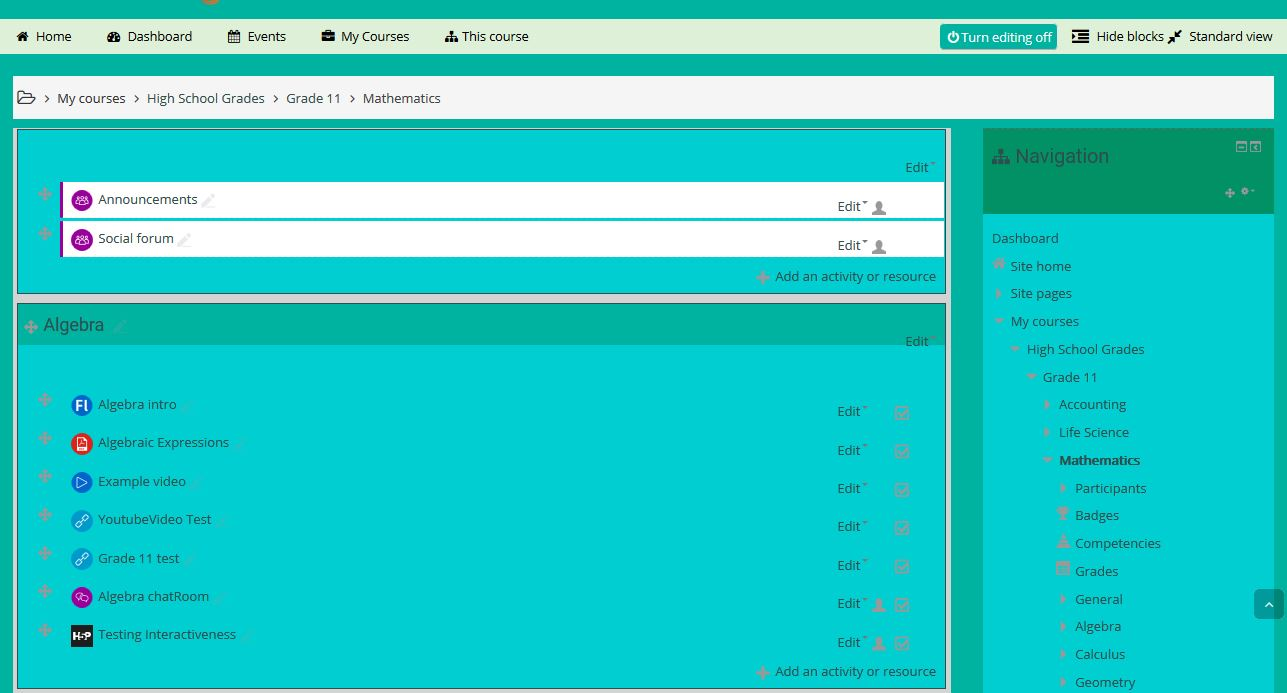
\includegraphics[width=1\textwidth]{images/editCourse.JPG}
			 	\caption{Turn on Editing}
			 	\label{Figure 7}
			 \end{figure}
	 		From hereon the teacher may click "add an activity or resource", here they will be exposed to all the possible content they can add. This is shown in Figure 8. You can then click "lesson" to add a lesson or "interactive content" to add a more interactive lesson. After this, click add to add the lesson. From hereon you will be taken to Figure 9 below.
	 	
	 		\begin{figure}[h]
	 			\centering
	 			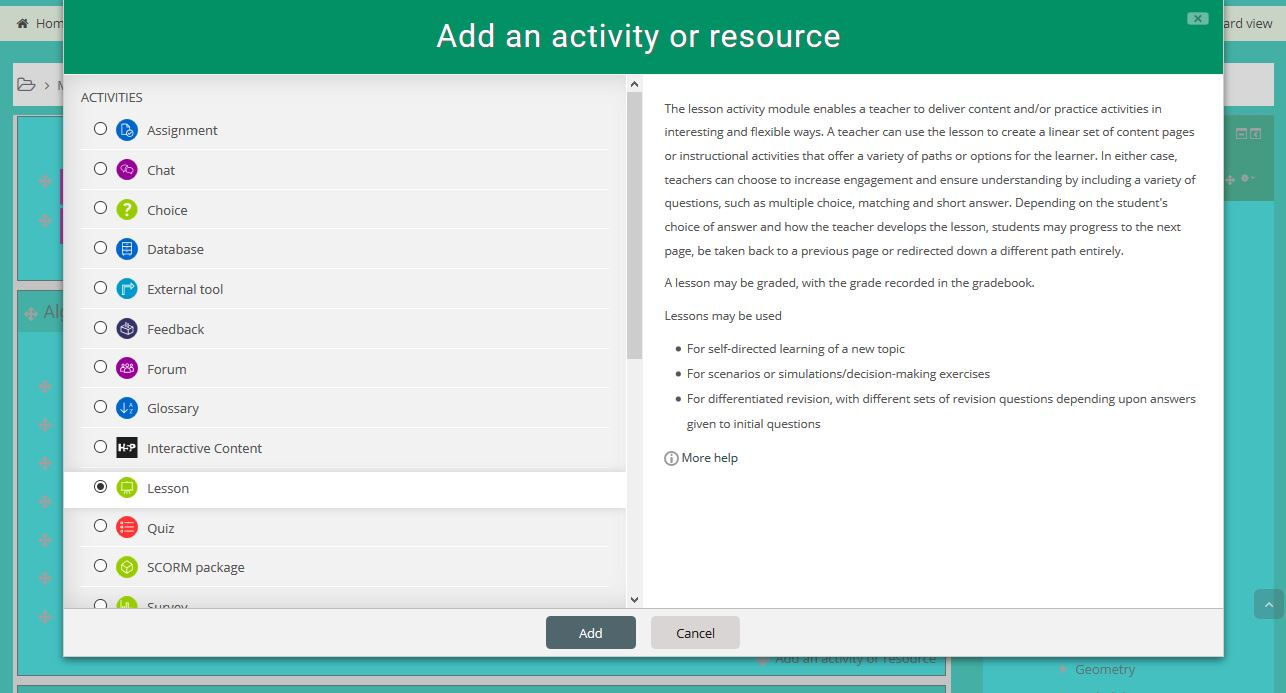
\includegraphics[width=1\textwidth]{images/addLesson.JPG}
	 			\caption{Add Lesson options}
	 			\label{Figure 8}
	 		\end{figure}
		 
%		 	\begin{figure}[h]
%		 		\centering
%		 		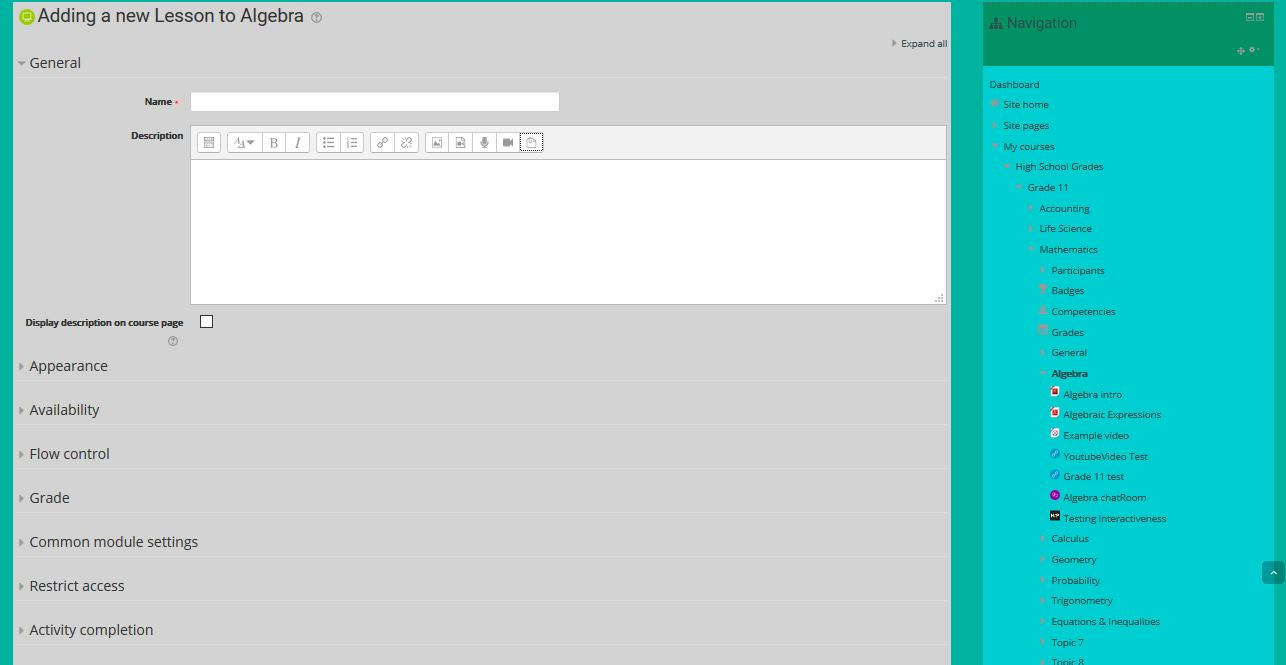
\includegraphics[width=1\textwidth]{images/completedLesson.JPG}
%		 		\caption{Add Lesson files}
%		 		\label{Figure 9}
%		 	\end{figure}
	 
	 		From here you will be shown all other possible options from how long the lesson should last to who it should be available to. Once finished with completing these, one can then save and return to the course page or view the lesson that was just added. 
	 	
	 	\subsubsection{Adding assessment activities(quizzes, assignments etc)}
	 		In order to add assessment activity, a teacher would follow exactly the same steps as adding a lesson above, however instead of clicking "lesson" on Figure 8, they can then just click the specific activity they wish to add, for instance "quiz",  and also proceed in a similar manner as Figure 8 below
%	\section{The Administrator}
%		 Also known as the superuser, this user will have all the powers of all the users, and will also be responsible for the addition, validation and removal of Expert and Marketing consultant accounts since these two users may be outsourced throughout the lifetime of the system.
		 

 	
 %	\section{Troubleshooting}
 %	 This section will be implemented at a later stage of the project.
 	 
 	 
% 	 	\section{Additional Information and Figures}
	
\end{document}